\documentclass[10pt,a4paper]{report}
\usepackage[utf8]{inputenc}
\usepackage[T1]{fontenc}
\usepackage{tabularx}
\usepackage{graphicx}
\usepackage{enumitem}
\usepackage{lmodern}
\usepackage{textcomp}
\usepackage{booktabs}
\usepackage{longtable}
\usepackage{titlesec}
\setcounter{secnumdepth}{4}
\usepackage{rotating}
\usepackage{array}
\usepackage{makecell}
\usepackage{multirow}
\usepackage[dvipsnames,table,xcdraw]{xcolor}
\usepackage{hhline}
\usepackage{caption}
\usepackage{verbatim}
\usepackage{longtable}
\usepackage[Lenny]{fncychap}
\graphicspath{{./Immagini/}}
\renewcommand*\contentsname{\textbf{Index}}
\usepackage{hyperref}
\hypersetup{colorlinks=true,linkcolor=black}
\usepackage{titletoc}
\usepackage{etoolbox}
\usepackage{lettrine}
\usepackage{geometry}
\geometry{
 a4paper,
 total={170mm,257mm},
 left=20mm,
 top=20mm,
 }
\makeatletter
\patchcmd{\chapter}{\if@openright\cleardoublepage\else\clearpage\fi}{}{}{}
\makeatother
\titleformat*{\section}{\centering\normalfont\Large\bfseries}

\begin{document}
\linespread{1,28}
\sffamily
\begin{titlepage}
\begin{center}
\normalsize

\begin{center}

\begin{tabular}[t]{@{} l @{} c @{} r @{}}
\parbox[c]{0.15\textwidth}{\raggedright 
\includegraphics[width=0.15\textwidth]{logo}}
&
\parbox[c]{0.7\textwidth}
{
\centering \bfseries
University of L'Aquila \\[-5pt]
\rule{0.6\textwidth}{1pt} \\
{\centering \scshape \small Department of Engineering and \\Information Science and Mathematics} \\}
&
\parbox[c]{0.15\textwidth}{\raggedleft 
\includegraphics[width=0.15\textwidth]{disim}}
\end{tabular}
\end{center}

\bigskip \bigskip



\bigskip
\bigskip
\bigskip

\vfil

{\bfseries \large
Report Homework \#1 \\}
{\bfseries \Large
Water Distribution, Leakage and Quality Control System
}

{\large
\bigskip
\bigskip
\bigskip
\bigskip
{\bfseries \large Professor \\ }
\bigskip
\textbf{Prof.} \textit{Vittorio Cortellessa} \\
}

{\large
\bigskip
\bigskip
\bigskip
\bigskip
{\bfseries \large Students \\ }
\bigskip
\textit{Gaetano Fichera \& Giovanni Lezzi} \\
}

\vfil
\vfil

\vspace{2\baselineskip}

{\large
\bigskip
\bigskip
\bigskip
\bigskip
{\bfseries \large Github Project Repository: \\ }
\bigskip
\textit{\href{https://github.com/GaetanoFichera/Water-Quality-Control-System}{https://github.com/GaetanoFichera/Water-Quality-Control-System}} \\
}

\vfil \vfil \vfil

\rule{\textwidth}{1pt}\\
{\scshape Academic Year 2017-2018}

\end{center}
\end{titlepage}
\tableofcontents{}
\chapter{\textbf{Light Rework On Our UML Model}}

After serious consideration of our last homework, we noticed that there were failures. Below is a list of rework:

\begin{itemize}
	\item We have applied the stereotypes to the Communication Paths 		within the Deployment Diagram;
	\item in order to improve system performance and to better 				stratify the deployment, we decided to add 3 new nodes: 
	\begin{itemize}
	\item "SeaweedPickingInlandControlUnit";
	\item "Seaweed Picking Outgoing Control Unit";
	\item "MagikarpControlUnit".
	\end{itemize}					 
	and , for this purpose we have also inserted a new profile called 		"Control Unit" from the	server 	stereotype, these 3 new nodes are 		connected to the server with a wired connection and to sensors 			with a wireless connection;
	\item For the connections between the Control Center Server and 		the	two Inland and Outgoing Seaweed Picking Control Units we 			have inserted a new communication path stereotype that does 			not consume resources because when we started the modeling 				work for the Queueing Network we considered the two Control 			Units located in the same physical space as the Control 				Center Server, then we use a "Internal Connection" stereotype with 	zero consumption of resources;
	\item We have added the operations to the components subsequently 		reused in the Sequence Diagram, not done in the first homework;
	\item we realized the lack of an internal server to the Control 		Center 	Pomezia that managed the requests coming from the App 			inside it;
	\item we realized that in the sequence diagram "check quality" the 	call from the component "check quality parameters inland /				outgoing" was missing to the component "parameters Quality 				archieve" to retrieve the desired water parameters;
	\item we have established the types of connections between one 			node and the other of the deployment diagram, obtaining:
	
	\begin{itemize}
		\item between the Control Center Server and the two Apps a 				Wired Connection;
		\item between Control Center Server and Seaweed Picking a 				Wireless Connection;
		\item between the Control Center Server and the Water Company 			Server and the Purification System Center an Internet 					Connection.
	\end{itemize}

	\item we have agreed that there is a single database that is 			connected to the water company server;
	\item we realized that in the water sampling phase, the sensors 		will send the data of the water samples to the Control Center 			Server which, in turn, using the sample archieve component will 		send the data to the water company server, the problem is that in 		the SD 	after the component sample archive is not invoked any 			component that refers to the water company server. Solution:
	\begin{itemize}
	\item We have decided to add a component called "Sample Archive" 		to the water company server which is responsible for saving data 		on the DB. In going to add this correction we realized 	that in			fact we have failed to use sample sender. Then we have made a 			small change: 
	\begin{itemize}
		\item sample sender is inside 	the control center server;
		\item sample archive is located inside the water company 				server and	manages the data on the db.
		\end{itemize}
	\end{itemize}	
	\item We modified the sequence diagram of "StartUpSamplingWater" 		as 	we realized that the component sample data on the 					SeadweedPIckingInland / Outgoing node communicated with the 			"SampleSender" component on the ControlCenterServer node.
\end{itemize}

Below you can find the description of the new profiles popping out.

\section{Wired Connection Profile}

\begin{longtable}{|p{4cm}|p{9cm}|}

\hline
\textbf{Wired Connection} & \\


\hline
Metamodel Class & Communication Path\\

\hline
Description & It is a representation of the physical meaning of Wired Connection\\

\hline
Tagged Values & \\

\hline
Constraints &\\

\hline
\end{longtable}
  
\section{Internet Connection Profile}

\begin{longtable}{|p{4cm}|p{9cm}|}

\hline
\textbf{Internet Connection} & \\


\hline
Metamodel Class & Communication Path\\

\hline
Description & It is a representation of the physical meaning of Internet Connection\\

\hline
Tagged Values & \\

\hline
Constraints &\\

\hline
\end{longtable}

\section{Wireless Connection Profile}

\begin{longtable}{|p{4cm}|p{9cm}|}

\hline
\textbf{Wireless Connection} & \\


\hline
Metamodel Class & Communication Path\\

\hline
Description & It is a representation of the physical meaning of Wireless Connection\\

\hline
Tagged Values & \\

\hline
Constraints &\\

\hline
\end{longtable}

\section{Internal Connection Profile}

\begin{longtable}{|p{4cm}|p{9cm}|}

\hline
\textbf{Internal Connection} & \\


\hline
Metamodel Class & Communication Path\\

\hline
Description & It is a representation of the physical meaning of Internal Connection\\

\hline
Tagged Values & \\

\hline
Constraints &\\

\hline
\end{longtable}

\section{Control Unit Profile}

\begin{longtable}{|p{4cm}|p{9cm}|}

\hline
\textbf{Internal Connection} & \\


\hline
Metamodel Class & Node\\

\hline
Description & It is a representation of the physical meaning of Control Unit\\

\hline
Tagged Values & \\

\hline
Constraints &\\

\hline
\end{longtable}
\chapter{\textbf{Identification Of Performance Requirements}}


The following consideration has been made: \\
one kilometer of the route with respect to the connection point with the system is taken into account for an Entry Water Channel or Exit of 5 meters radius, and every 10 meters must be 10 Seaweed Picking, with a total of 1000 Seaweed Picking. \\
Non-functional requirements are:
\begin{itemize} 
	\item Each sensor must take 10 ms to carry out a sampling;
		\item The time between a sampling and an other is 60 s;
	\item The Utilization of each node must be less than 90\%;
	\item The response time of an Actor Task must not exceed 300 ms specifically referenced to "CheckWaterQuality" Use Case.
\end{itemize} 

\newpage \chapter{\textbf{Model WCS With Execution Graphs}}

The Use Cases we have considered are:
\begin{itemize}
\item UC1 StartUp Sampling Water activated by Sample Supervisor;
\item UC3 Check Water Quality activated by Quality Control Supervisor.
\end{itemize}
In reference to the Use Cases taken into consideration, to better understand our architecture, we have combined the Deployment Diagram with Component Diagram. In the figure below this is represented.

\begin{center}
  \makebox[\textwidth]{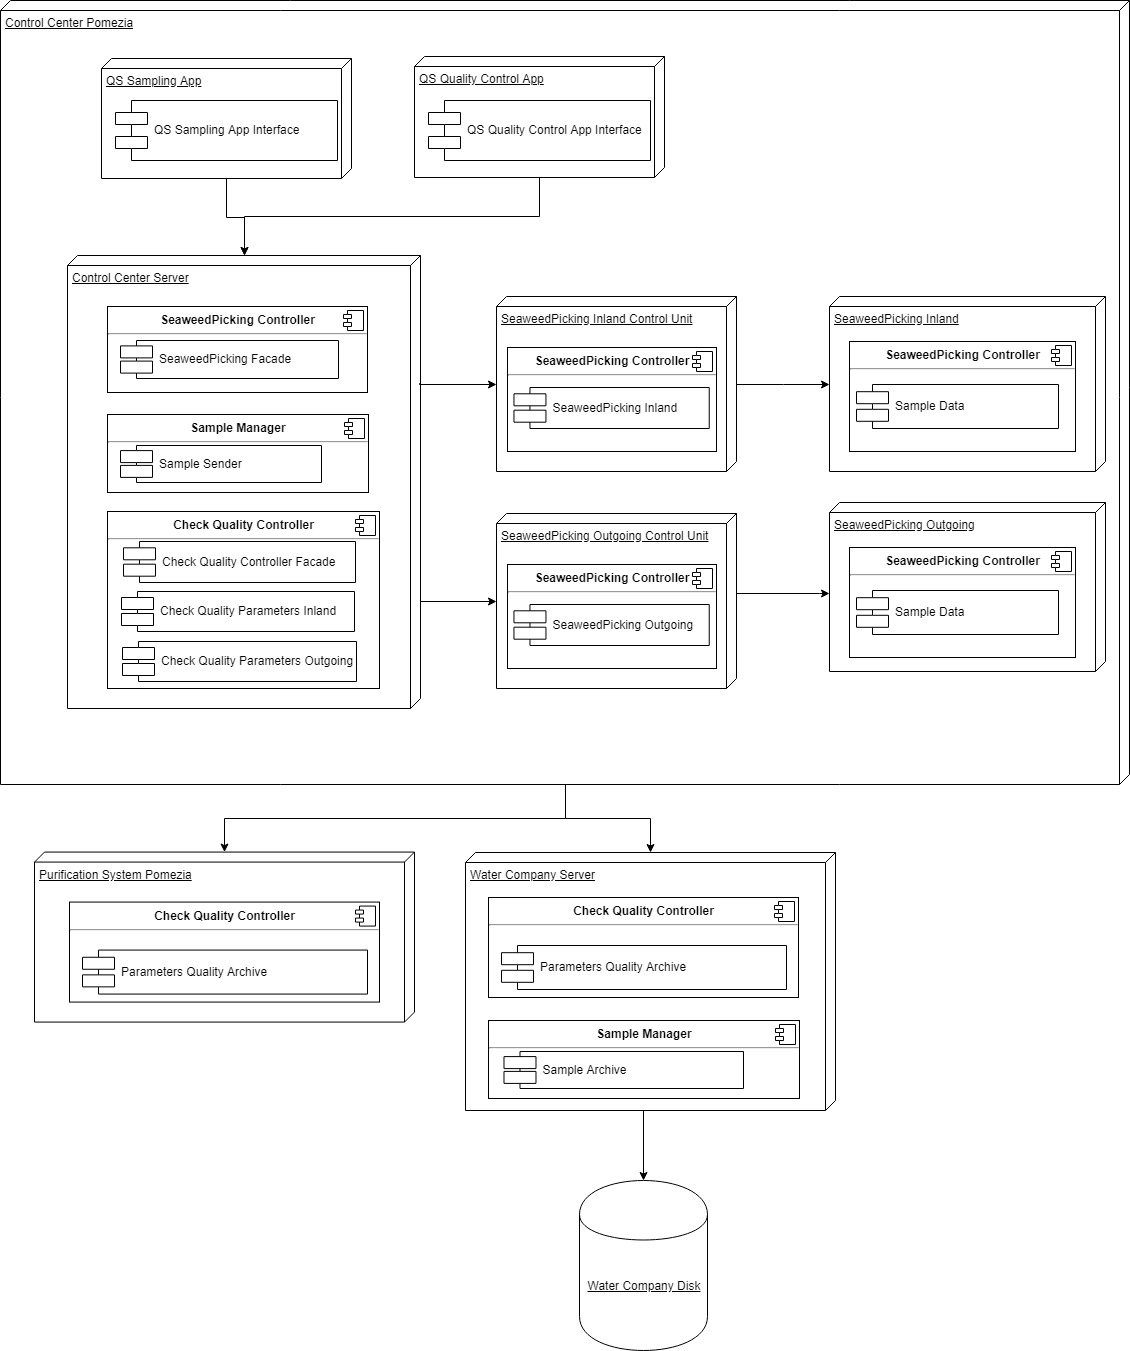
\includegraphics[width=\textwidth]{DeploymentDiagramEComponentDiagram.jpg}}
\end{center}
\bigskip
\captionof{figure}{Deployment Diagram + Component Diagram}

\newpage \section{Demand Vector}

Il Demand Vector scelto in base alle risorse virtuali che risaltano dal deployment diagram sono: 

\begin{longtable}{|p{4cm}|p{9cm}|}

\hline
\textbf{
Wired Connection Request} & \\

\hline
\textbf{Wireless Connection Request} & \\

\hline
\textbf{Internet Connection Request} & \\

\hline
\textbf{Database Request} & \\

\hline
\textbf{Control Center Server CPU} & \\

\hline
\textbf{Water Company Server CPU} & \\

\hline
\textbf{Purification System Pomezia CPU} & \\

\hline
\textbf{Seaweed Picking Inland Control Unit CPU} & \\

\hline
\textbf{Seaweed Picking Outgoing Control Unit CPU} & \\

\hline
\textbf{Seaweed Picking Outgoings Sample Request} & \\

\hline
\textbf{Seaweed Picking Inlands Sample Request} & \\

\hline
\end{longtable}

\textbf{Spiegare cosa sono queste risorse virtuali}\\
\newpage

The Execution Graphs obtained are:

\begin{itemize}
\item UC1 Sampling Water activated by Sample Supervisor:
	\bigskip
	\bigskip
	\begin{center}
 	 \makebox[\textwidth]{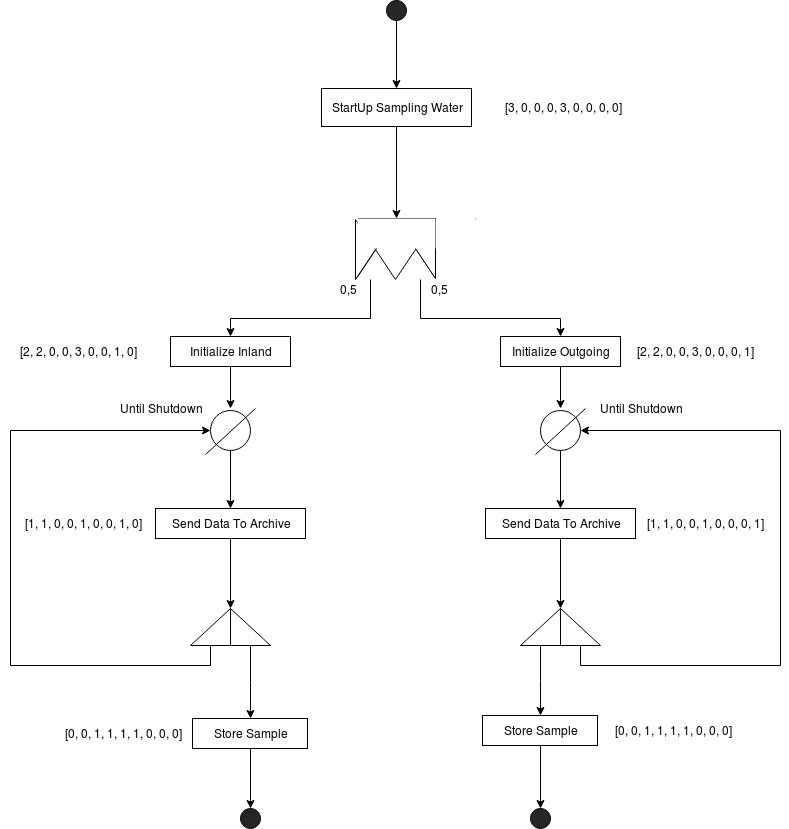
\includegraphics[width=\textwidth]				{EGUC1StartUpSamplingWater.jpg}}
	\end{center}
	\bigskip
	\captionof{figure}{EG UC1 StartUp Sampling Water}
\newpage
\item UC3 Check Water Quality activated by Quality Control Supervisor:
	\bigskip
	\bigskip
	\bigskip
	\bigskip
	\begin{center}
 	 \makebox[\textwidth]{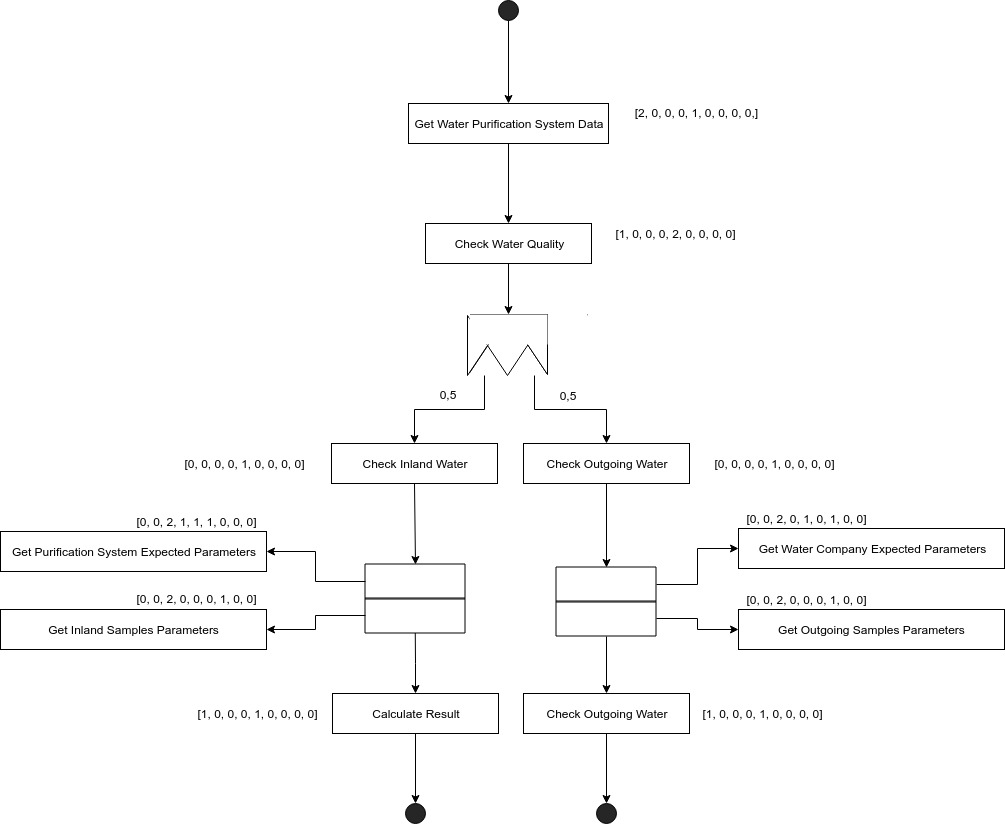
\includegraphics[width=\textwidth]				{EGUC3CheckWaterQuality.jpg}}
	\end{center}
	\bigskip
	\captionof{figure}{EG UC3 Check Water Quality}
\end{itemize}




\newpage \chapter{\textbf{Queueing Network Model}}

Then we have identified the physical nodes of our system going to introduce how the Execution Graphs are connected to them:
\bigskip
\bigskip
\bigskip
\bigskip
\begin{center}
\makebox[\textwidth]{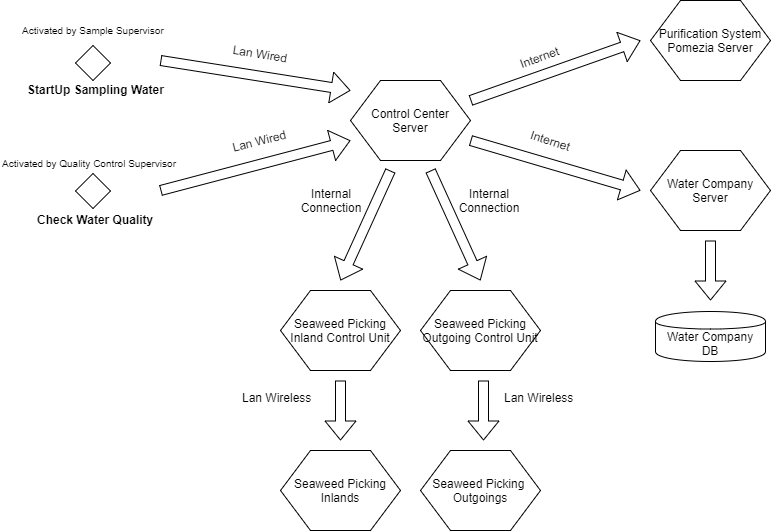
\includegraphics[width=\textwidth]				{PhysicalNodes.png}}
\end{center}
\bigskip
\captionof{figure}{Physical Nodes}

\newpage
This is the Queueing Network so obtained:
\bigskip
\begin{center}
\makebox[\textwidth]{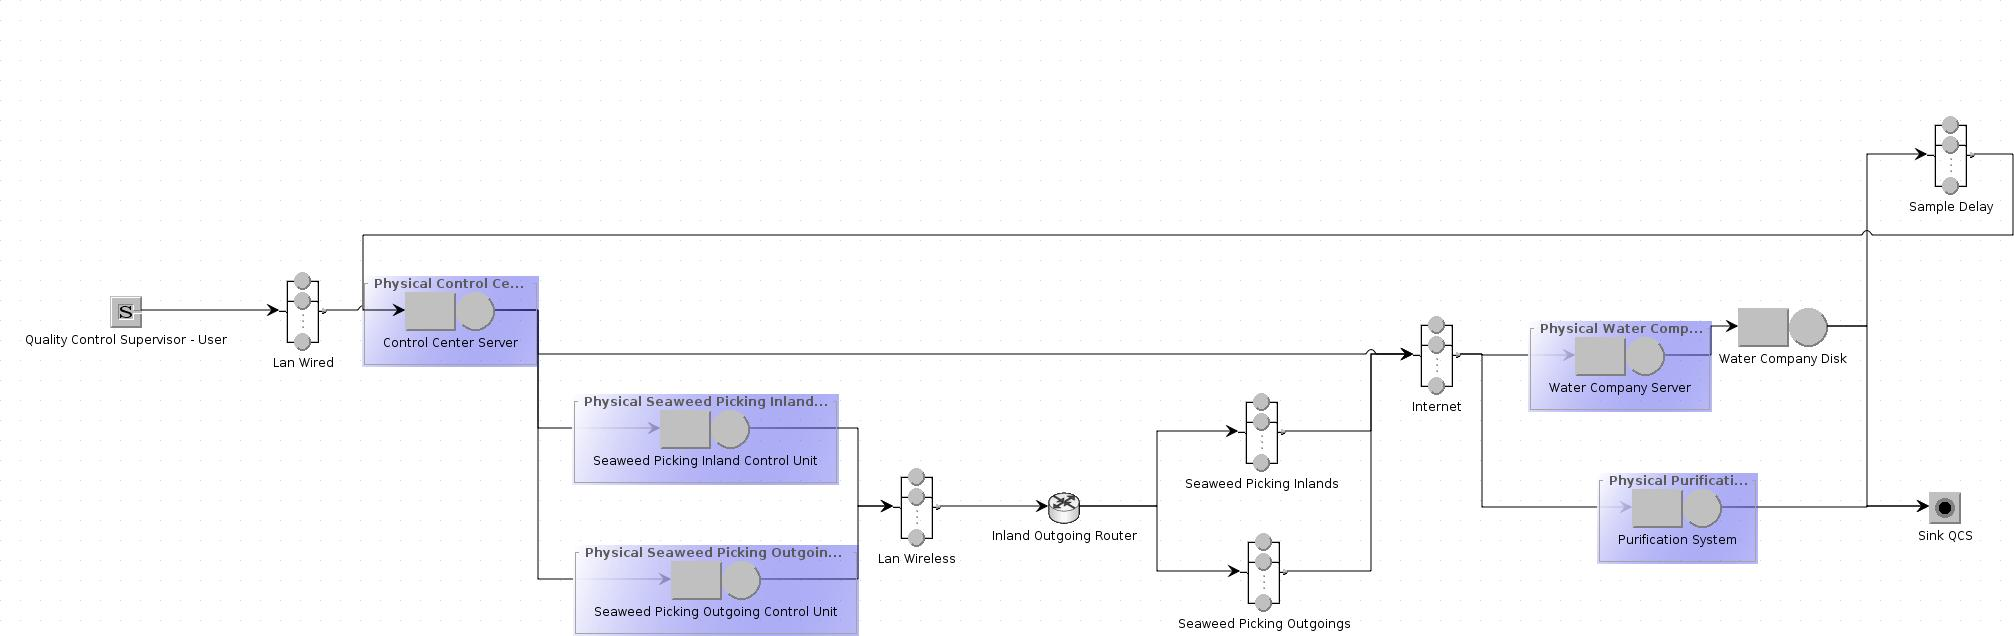
\includegraphics[width=\textwidth]				{QueueingNetwork.jpg}}
\end{center}
\bigskip
\captionof{figure}{Queueing Network}

\bigskip
After several tests, we agreed to reduce the sampling time to 500 seconds to refine the performance analysis. On jmt for the same reason we have only one SeaweedPicking Control Unit and no two for In / Out.\\
We have also decided to eliminate the finite capacity regions as useless for the purposes of our project. So our final Queueing Network has become this:
 
\bigskip
\bigskip
\bigskip
\begin{center}
\makebox[\textwidth]{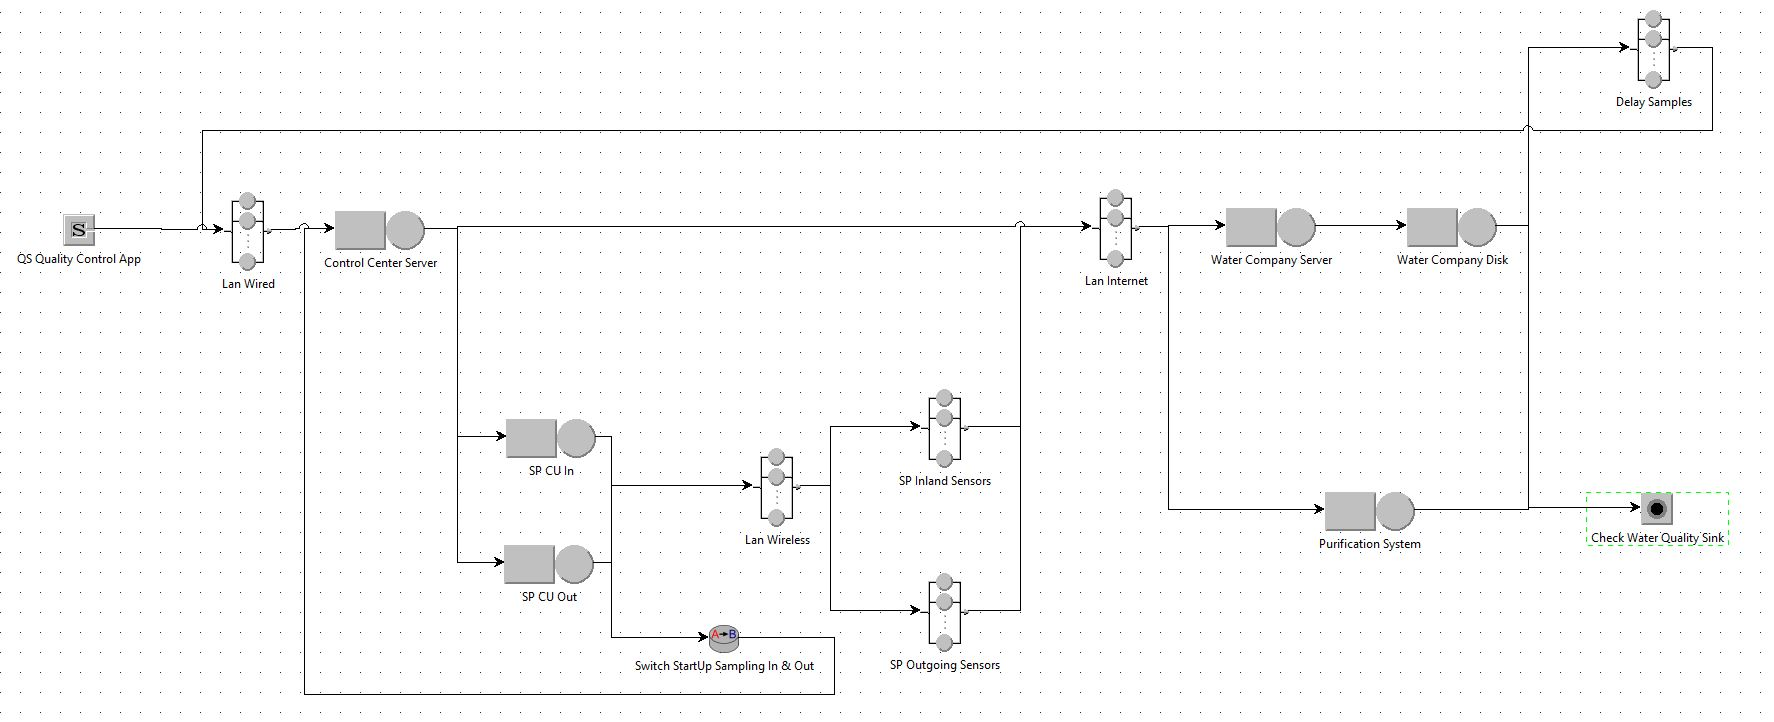
\includegraphics[width=\textwidth]				{QueuingNetworkFinal.jpg}}
\end{center}
\bigskip
\captionof{figure}{Final Queueing Network}
\end{document}